% Déclaration du type de document (report, book, paper, etc...)
\documentclass[a4paper]{paper} 
 
% Package pour avoir Latex en français
\usepackage[utf8]{inputenc}
\usepackage[T1]{fontenc}
 
% Quelques packages utiles
\usepackage{listings} % Pour afficher des listings de programmes
\usepackage{graphicx} % Pour afficher des figures
\usepackage{amsthm}   % Pour créer des théorèmes et des définitions
\usepackage{amsmath}
\usepackage{microtype} % Optical margins FTW
\usepackage{url}
\usepackage{booktabs} % Allows the use of \toprule, \midrule and \bottomrule in tables for horizontal lines
\usepackage[per-mode=symbol]{siunitx}
\usepackage{floatrow}
\usepackage{caption}
\usepackage{subcaption}
\usepackage{mhchem}
\usepackage[acronym,smallcaps]{glossaries}


% Début du document
\begin{document}
\begin{titlepage}

\newcommand{\HRule}{\rule{\linewidth}{0.5mm}} % Defines a new command for the horizontal lines, change thickness here

\center % Center everything on the page 
%----------------------------------------------------------------------------------------
%	HEADING 
%----------------------------------------------------------------------------------------
\textsc{\LARGE Club Vaudois de Robotique Autonome}\\[1.5cm] 

%----------------------------------------------------------------------------------------
%	TITLE 
%----------------------------------------------------------------------------------------
\HRule \\[0.4cm]
{ \huge \bfseries Eurobot 2014 : Pilot Study}\\[0.4cm] % Title of your document
\HRule \\[1.5cm]
 
%----------------------------------------------------------------------------------------
% LOGO EPFL
%----------------------------------------------------------------------------------------
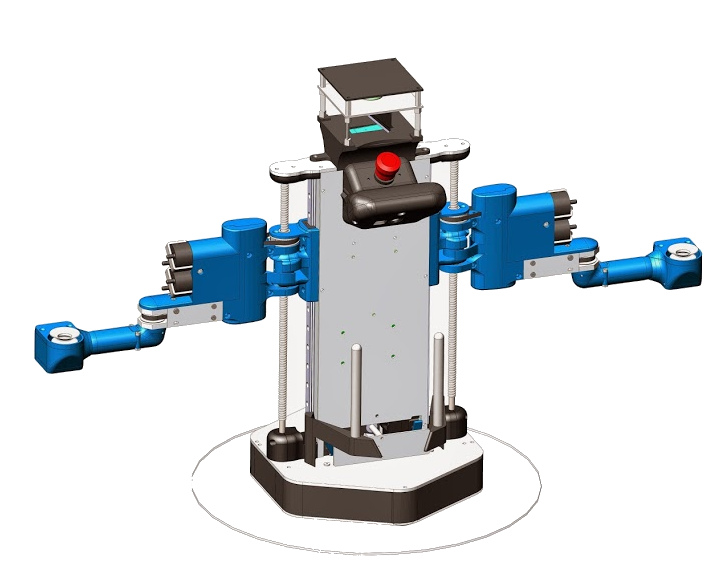
\includegraphics[width=\textwidth]{images/Debra_IV_1}\\[2cm] 

%----------------------------------------------------------------------------------------
%	AUTHORS 
%----------------------------------------------------------------------------------------

\vfill % Fill the rest of the page with whitespace

{\large \today}
\end{titlepage}



\tableofcontents

\section{Summary}

% TODO document ici
\section{Experiment 1}
Lorem ipsum test

\section{Experiment 2}
Lorem ipsum test

\end{document}
